\documentclass{article}

\usepackage[english]{babel}

% Set page size and margins
% Replace `letterpaper' with `a4paper' for UK/EU standard size
\usepackage[letterpaper,top=2cm,bottom=2cm,left=3cm,right=3cm,marginparwidth=1.75cm]{geometry}
\usepackage{graphicx}
\usepackage{xcolor}
\usepackage[colorlinks=true,linkcolor=blue,citecolor=red]{hyperref}

\hypersetup{
    colorlinks=true,
    linkcolor=blue,
    citecolor=pink,
}

\title{Research Automation White Paper}
\author{Shiro Takagi}

\begin{document}
\maketitle

\section{What is Research?}

\subsection{The Working Definition of Research}
Research is the act of generating new knowledge. In other words, it can be thought of as an endeavor to make the unknown known.

\subsection{The Patterns in Research}

It is believed that research began with individual and concrete tasks. Among them, common actions were patterned and crystallized as a scientific method. We currently recognize this abstract set of behaviors as research. For example, hypothetico-deductive method and hypothesis testing are abstracted scientific method.

Also, researchers use a research paper as a medium of knowledge transfer. Therefore, there are patterned activities related to a research paper. Examples of these include conducting surveys, gathering information from papers, and writing a thesis.

Note that these are necessary tasks just because we use a paper as a medium of knowledge transfer, but they may not necessarily be indispensable for generating new knowledge. There are other such tasks as well. For example, peer review and fund raising are essential to current research practices in society, but they may not necessarily be indispensable for knowledge production.

In this way, various tasks arise in conjunction with research. When considering the automation and optimization of research, it is desirable to consider streamlining all of these tasks. However, in this article, we focus on the process from determining a research topic to publishing a research paper. We will refer to this process simply as the \textit{research process} from here on.

\subsection{Research Process}

\subsubsection{Overview}

As mentioned earlier, research is an attempt to turn the unknown into the known. Therefore, the research process can be seen as a function that takes the unknown as input and outputs the known. However, in reality, a single research paper may not be enough to turn the unknown into the known. Therefore, in practice, the research process is considered to be a procedure that takes the unknown as input, and outputs a text that describes the procedures and their results, as well as their interpretation, in order to turn the unknown into the known.

First, let me structure the common research process. In particular, I will base the structuring of the research process on the method of empirical science, which many researches rely on as a foundation. However, I believe that this framework can be applied to other research activities, such as mathematics, as well. I will explain the reason for this later.

The research process, especially that of empirical science, is carried out through the following steps: topic decision, hypothesis generation, verification design, verification, and analysis of experimental results. The outputs of these steps are then written into a paper, which undergoes peer review and is eventually published.

Note that some commonly seen items, such as surveys, are not included here for a reason. First, as mentioned earlier, gathering information from papers is only a means of knowledge transfer through the use of a thesis. Second, information extraction from papers can be done at any stage of the research process. Thus, I believe that processing related to a paper, such as \textit{reading papers} and \textit{writing a paper}, needs to be considered separately from the aforementioned research process.

Taking all of this into account, the research process can be expressed as follows:

\begin{figure}[htb]
    \centering
    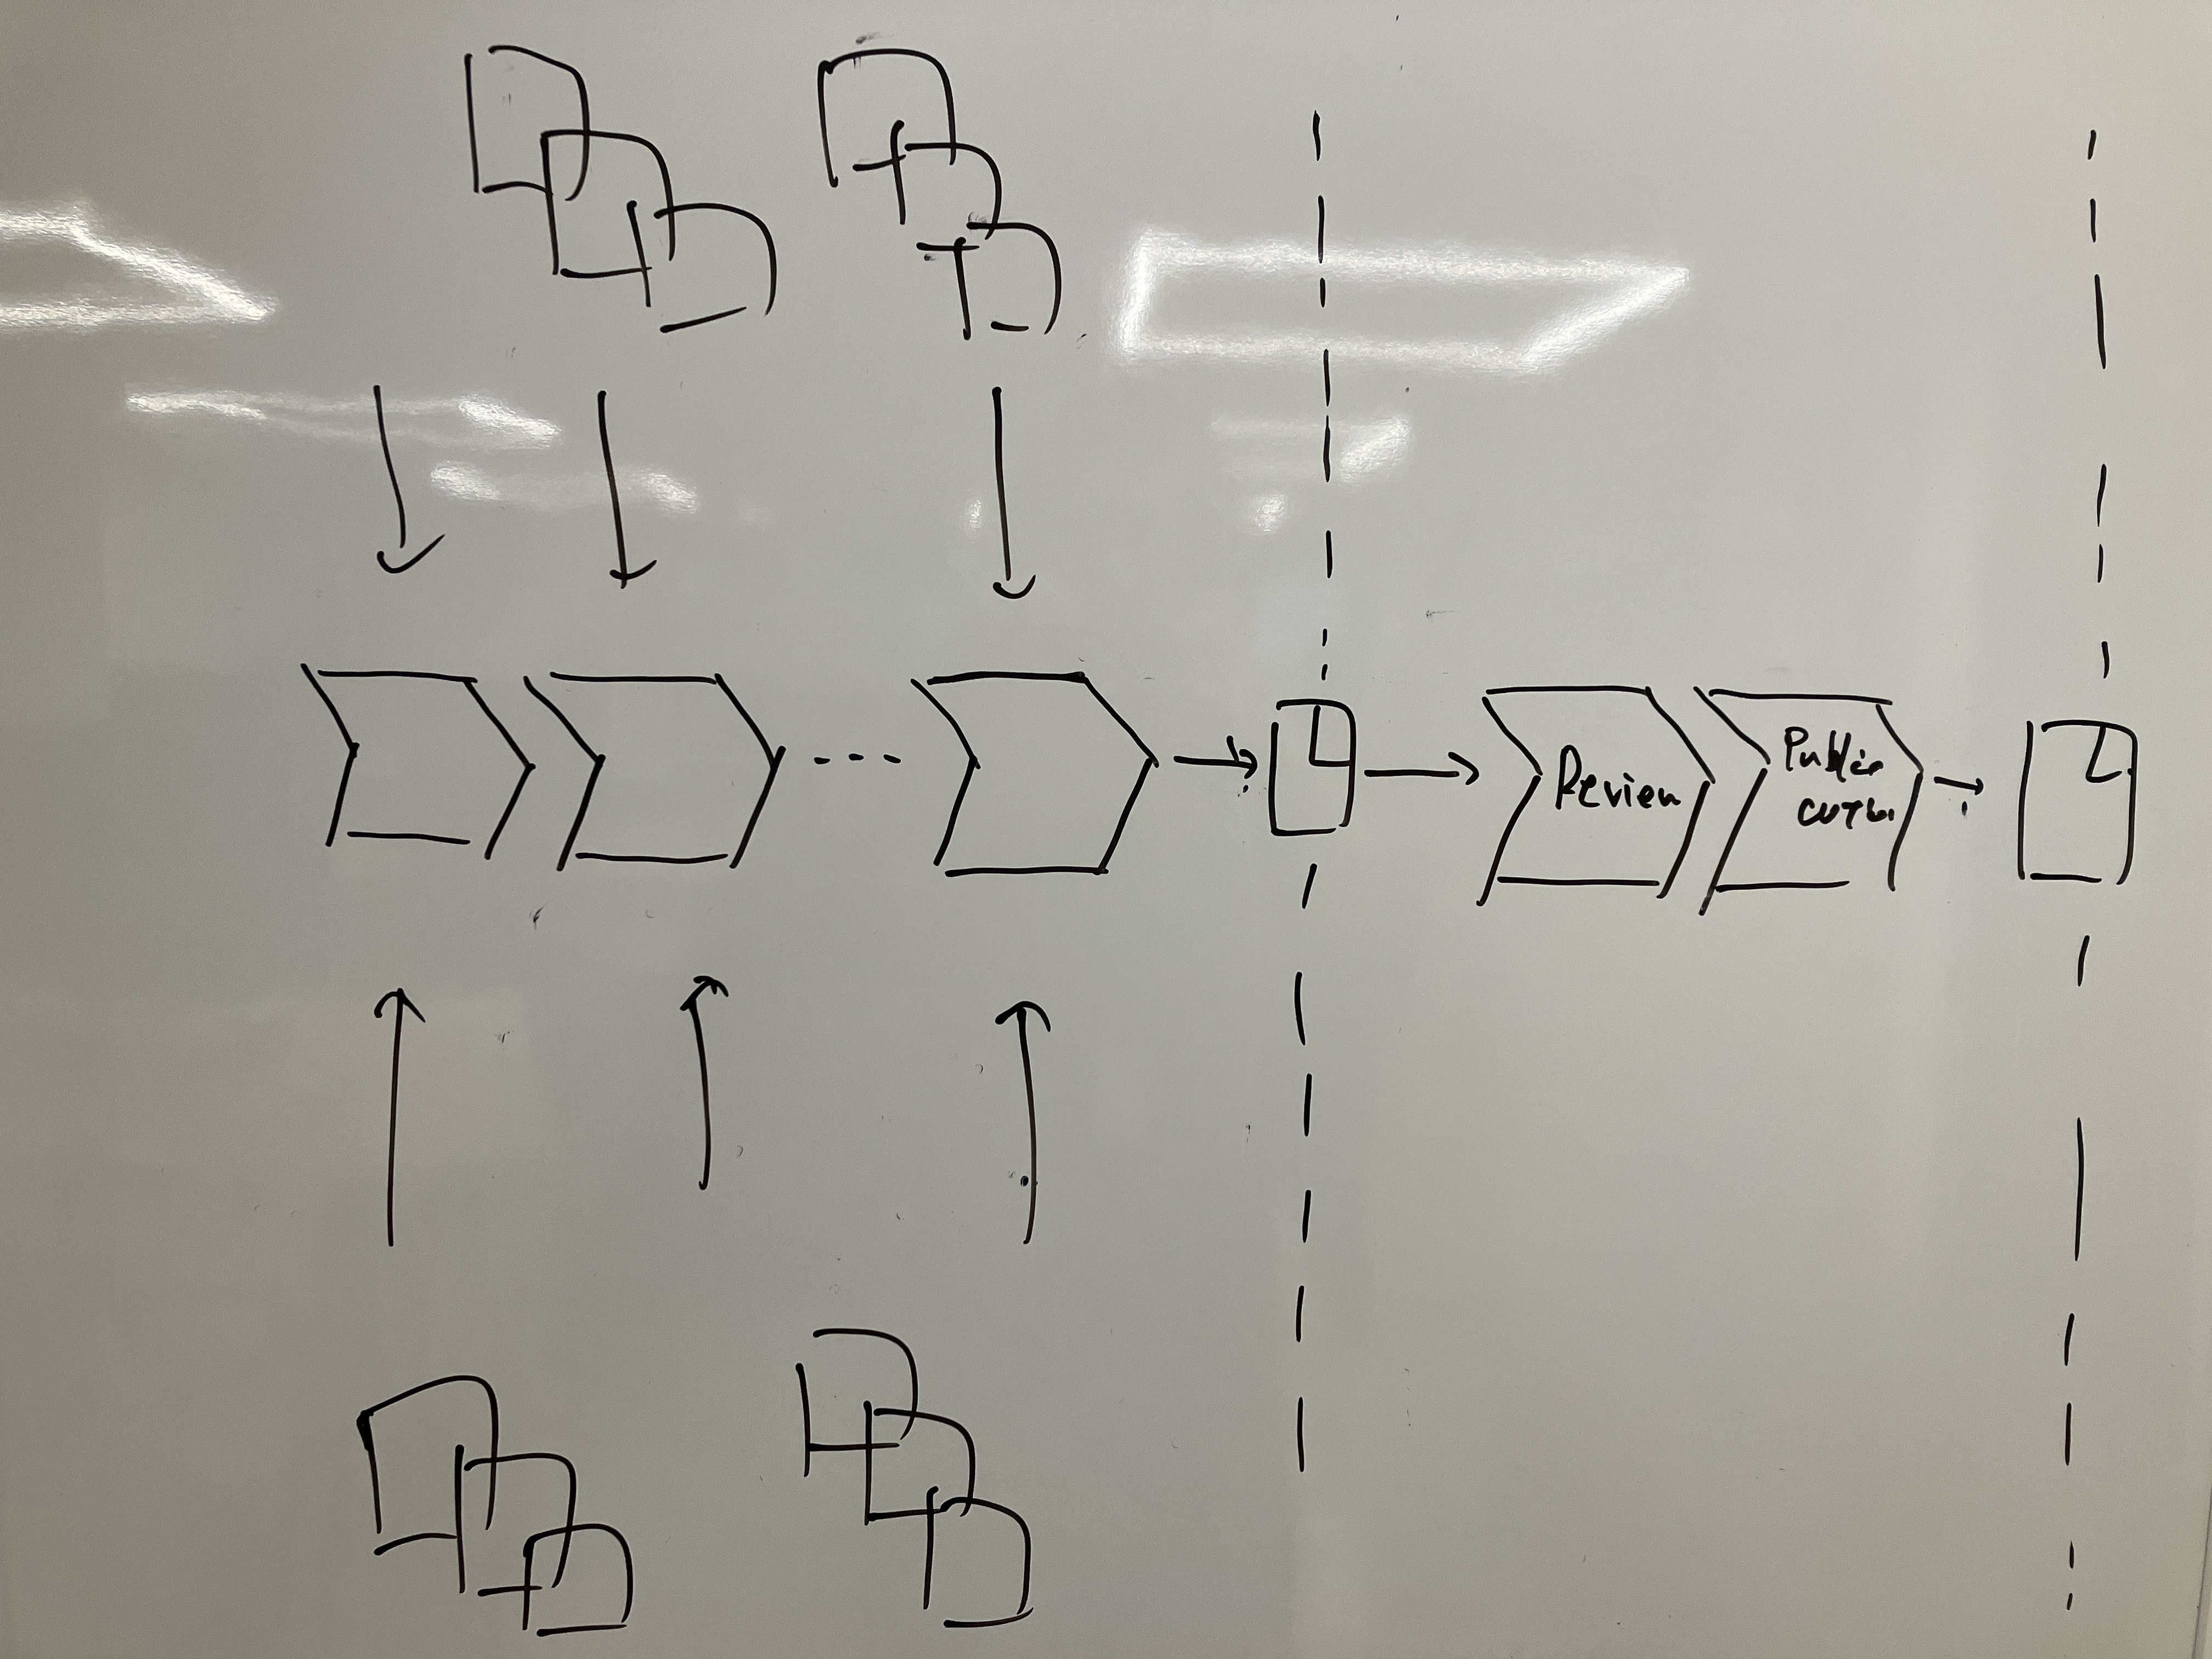
\includegraphics[width=\textwidth]{figs/researchprocess.jpg}
    \caption{Caption}
    \label{fig:research_process}
\end{figure}

This structuring is tentative and there may be a better way to structure the research process. However, I have created this structure for practical purposes in order to move the discussion forward. I will explain the reason for this division later. It is extremely important to consider research and, ultimately, the automation of research when thinking about better structuring. I hope the structure of this article be a starting point for conceiving a better structurization.

I will now proceed to a more detailed explanation of each step in the structured research process, followed by a separate discussion on reading and writing research papers.

\subsubsection{Topic Decision}
As mentioned earlier, research is an act of creating new knowledge. Usually, when people engage in research, they have a specific \textit{purpose} in mind before they decide what unknown they try to make known.

For example, let's say that someone proposes an algorithm that extends the reasoning capabilities of neural networks. This research may entails the thought process of ``I want to create artificial general intelligence, which requires reasoning capabilities, and for that we need to....'' In this case, the final purpose is to achieve ``artificial general intelligence'', and the research conducted as a result is ``proposing an algorithm that extends the reasoning capabilities of neural networks.'' Of course, this purpose may also be a means to achieve another purpose (such as intellectual curiosity), but since we cannot infinitely regress, we will assume that there is one purpose for one study.

In any case, there is gap between the purpose and the unknown we are trying to make known. We connect the sub-goals (, or sub-unknowns) by multi-step plausible inferences process.

\begin{figure}[htb]
    \centering
    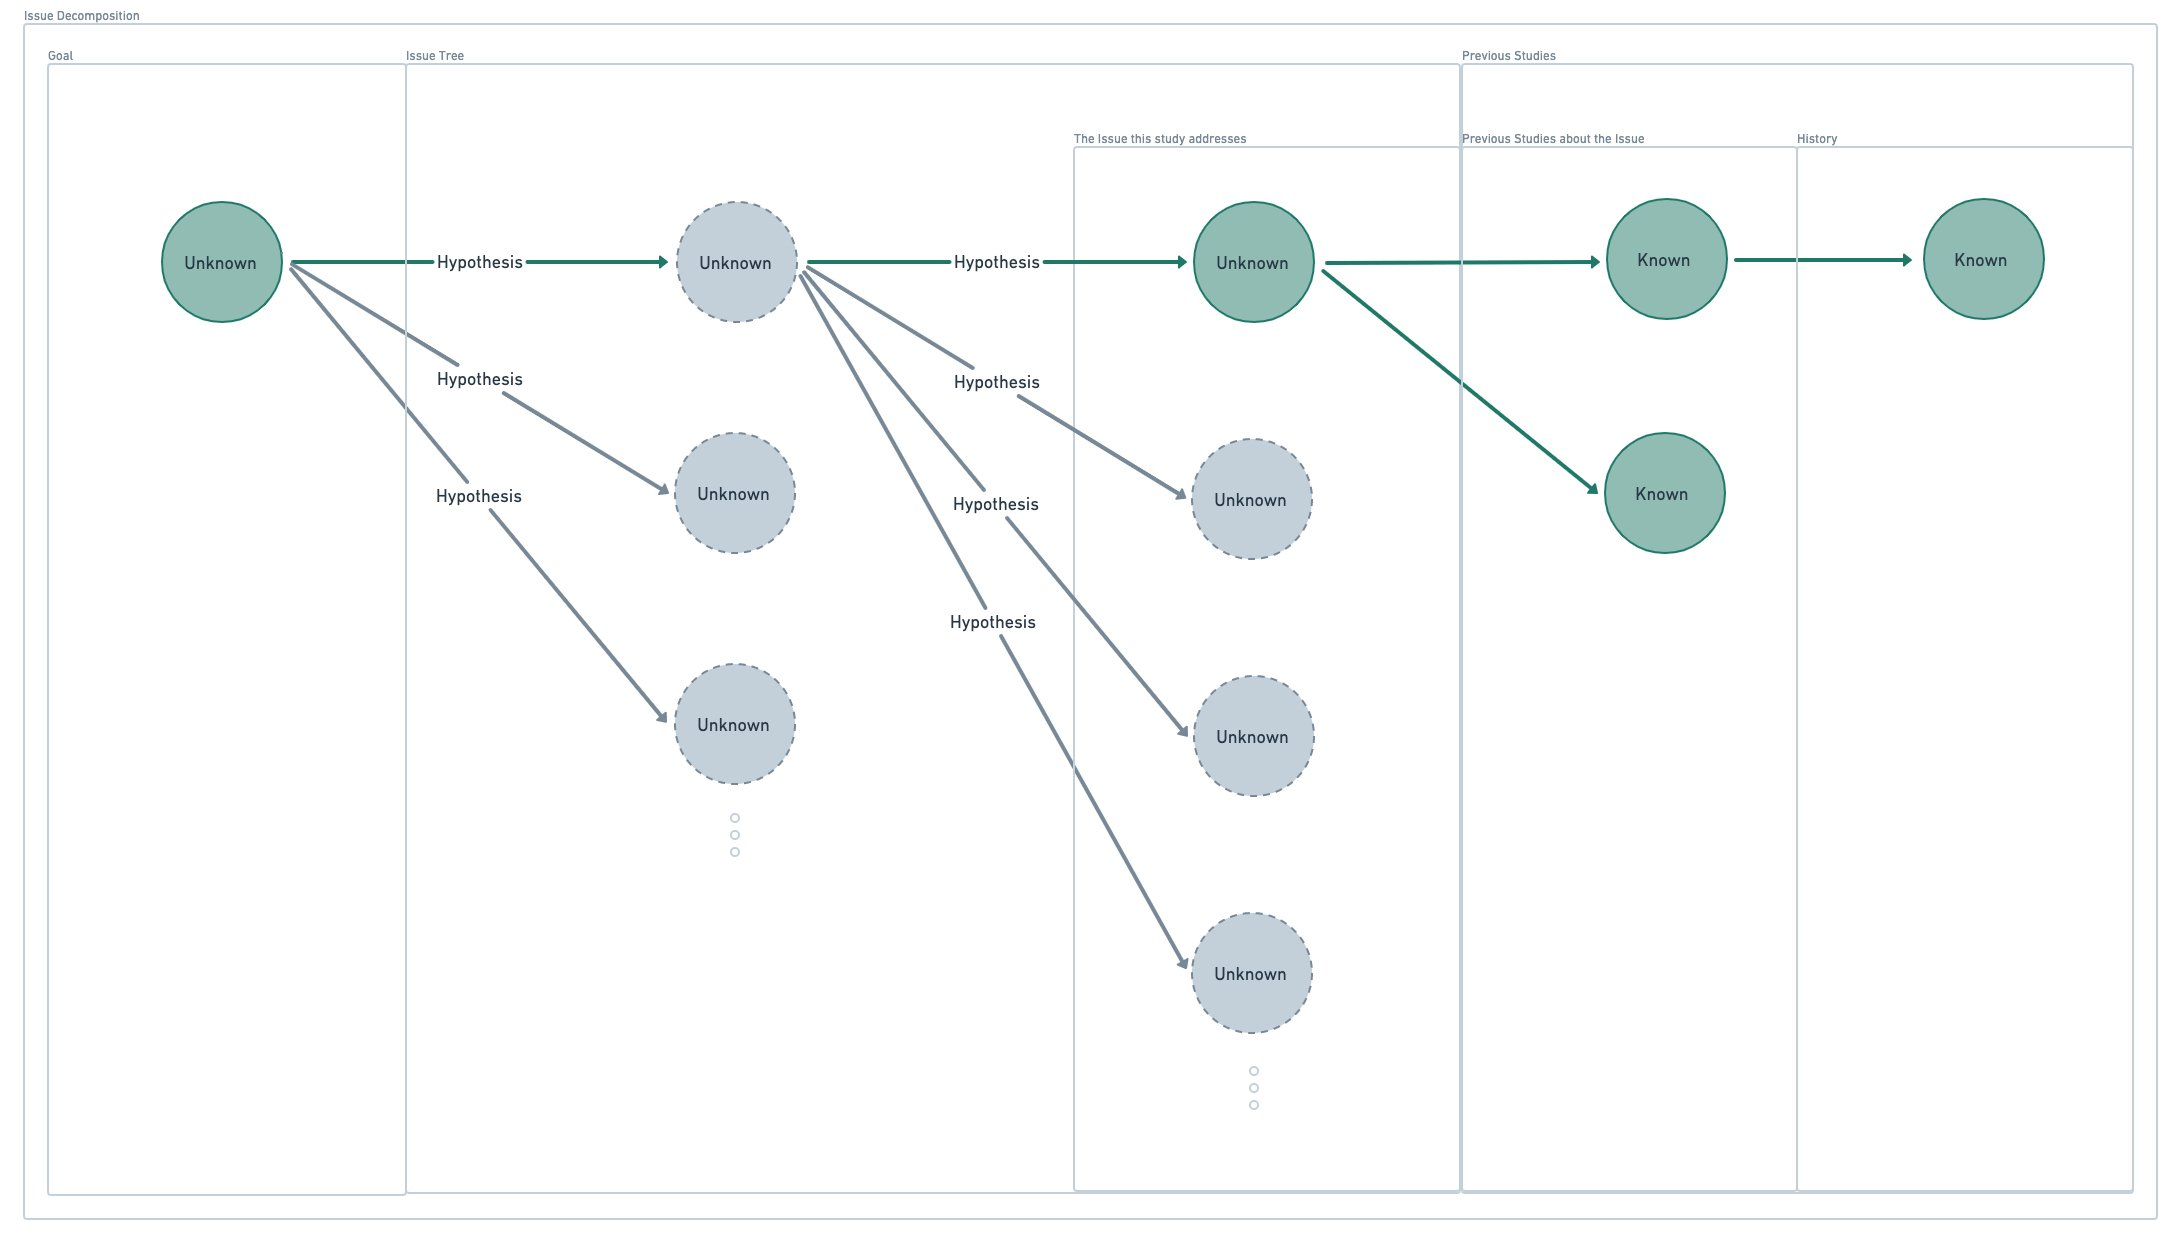
\includegraphics[width=\textwidth]{figs/unknown_tree.jpeg}
    \caption{Caption}
    \label{fig:unknown_tree}
\end{figure}


In other words, when humans engage in research, topic selection and issue identification are necessary.

\subsubsection{Hypothesis Generation}
Once the problem to be addressed has been identified, the next step is to generate a hypothesis. Research is an act of producing new knowledge, which can also be described as the act of converting the unknown to the known. Therefore, in research, inference about the unknown is inevitable. 

The scientific method, a methodology for knowledge production as previously mentioned, predominantly employs the hypothesis testing method. In this approach, a prediction about the unknown is explicitly stated as a hypothesis, and a procedure called verification is established to evaluate the validity of this hypothesis. Through this verification process, the evaluation of the hypothesis is conducted and the uncertainty towards the target unknown is reduced. This is the knowledge production based on the hypothesis testing method.

Hypotheses are often implicitly established even if they are not explicitly stated. Moreover, multiple hypotheses are often created in a study. For example, in mathematics, knowledge production is achieved through a deductive process called proof. However, when searching for lemmas to use in this process, we sometimes make predictions such as ``this lemma might be useful`` and examine it with specific examples. This may be considered as implicitly establishing a hypothesis and roughly verifying it. Therefore, even if the hypothesis testing method is not explicitly utilized, hypothesis generation is considered to be a very important part of research in nature.

In engineering research, as part of new knowledge, it is often required to propose actual design plans or algorithms. This can be considered as having a similar function to a hypothesis in the sense that it is a proposal for addressing a problem and is evaluated in some way.

In mathematical research, proving a theorem that was previously unknown is the production of knowledge. However, since mathematics is a deductive system, if the proof is correctly executed, it can be said to be ``correct'' in that sense. In other words, the proof itself is both the proposal and the verification. Therefore, mathematics is not a type of work that separates hypothesis and verification.

\subsubsection{Verification Design}
Once a hypothesis has been established, a verification plan is created to determine how to verify it. The specific method of verification depends on the subject being investigated, making this aspect of research difficult to structurize and automate in a unified way.

However, in many empirical sciences, the likelihood of a hypothesis is evaluated based on statistical significance. This is done by \textit{hypothesis testing} in practice. As this is a hypothesis test, it can only reject the null hypothesis, rather than directly determining the correctness of the hypothesis. Therefore, it can only be said that the hypothesis has survived for the time being. The belief that the surviving hypothesis is more likely to be valid is the basis for decision-making.

In any case, humans seem to use statistics or probability as the basis for assessing the validity of a hypothesis. In other words, we seem to concede to consider a hypothesis as plausible if something that cannot happen by chance, such as observing the same number repeatedly. This is based on the assumption of the ``principle of confirmation,`` which assumes that if the number of observations increases, it can be considered more reliable, and the ``principle of uniformity,`` which assumes that things will continue to proceed as they have been if the conditions remain the same. These beliefs ultimately serve as the basis for verification and scientific knowledge production. 

I will not delve into the validity of these beliefs here. What matters is that our research activity follow a practice that ``when a hypothesis is present, and a certain criterion and procedure are prepared, and the hypothesis is considered valid according to that procedure, we consider it valid.''

In theoretical research, sometimes there is no verification plan. Theory is a hypothesis, and its validity is determined separately through verification (not in the sense of whether it is mathematically valid, but for example whether it explains physical phenomena or not). However, in complex modern science, theorists propose a theory, and experimentalists verify it.

% Therefore, it is understood that in current research practice, shared knowledge in the form of papers may not necessarily provide a complete answer to a given question. This is similar to research on negative data. Negative data cannot solve the unknown initially declared, but it can reduce a certain degree of uncertainty towards it. This is because the validity of the presented hypothesis may have decreased somewhat. If this is the case, each research shared in the form of a paper may be more appropriate to describe as "reducing uncertainty towards the unknown," rather than "making the unknown known." This can become complicated when scrutinized strictly, so let's put this aside for now and continue to discuss how "producing new knowledge" is research.

In reality, conducting research is expected to be done with limited resources (time, funding, computing resources, people, etc.). Therefore, it is necessary to consider these resources when determining the verification approach. After a research design is determined at an abstract level, the feasibility of the research plan is roughly evaluated through a simple problem setting. This is known as a pilot study.
\subsubsection{Verification}

As mentioned earlier, in the case of empirical sciences, testing is often performed. Therefore, data is first generated, processed, and finally verified using the processed data. If we summarize the process of generating and processing raw data as data generation, this process can be broadly divided into data generation and judgment based on verification criteria. It may be rather said that the act of research itself is a process of repeatedly generating data and performing some kind of processing on it.

I separated the verification plan from the verification because I want to separate the description and execution of the process. The verification plan is analogous to coding, while the verification is more similar to executing the code.

The output of this process is usually wrtitten in the result section in the paper.

\subsubsection{Analysis}
At this stage, researchers interpret the results obtained from the verification. While the process leading up to the verification involved following a pre-determined procedure, researchers now consider implications that may relate to the unknown that they originally attempted to solve. For example, they contemplate whether the hypothesis has been rejected or the claim has been supported, and whether there are any other noteworthy points to consider. In papers, this stage is often described in discussion section.

\subsubsection{Peer Review}
In current research, a small group of experts review papers and the results that pass through their review are published. The review evaluates papers from multiple different perspectives. For example, at NeurIPS 2022, papers are evaluated based on the criterias of originality, quality, clarity, and significance.

\subsubsection{Searching}
Research is an endeavor to create knowledge based on existing studies. Therefore, the first step is to search for papers that should be read. In this article, we refer to this process as \textit{search}.

To find the necessary papers, you have to know what is written in each paper. Therefore, \textit{search} is closely related to \textit{reading}, which will be discussed in the next section. Here, For convenience, we will distinguish between the two: the former refers to finding the necessary papers from a large collection of papers, and the latter refers to extracting necessary information from the obtained single paper.

I shall make mention of the relationship between these concepts and the activity commonly referred to as a \textit{survey}. I define the survey as a series of processes of 1. searching for necessary papers, 2. extracting information from multiple papers, and 3. comparing them to make some kind of decision. Please note that comparison, searching, and reading are all closely related to each other in this context as well; for instance, proper comparison between papers is necessary for better searching.

The distinction between the aforementioned tasks of reading and searching, as well as the definition of survey, are based solely on the fact that we humans distinguish between them. However, if desired information could be directly obtained through natural language instructions from a large set of academic paper data, the tasks of searching, reading, and comparison would become an end-to-end process. Thanks to the remarkable development of large-scale language models in recent years, such a possibility has become a realistic one. Further details on this possibility will be discussed later.

\subsubsection{Reading}
As previously mentioned, acquiring information from academic papers is a fundamental task necessary in all aspects of research.

In particular, there may be cases where one does not even know where to find the necessary knowledge. Therefore, in order to obtain the required information, it is necessary to first search for the academic papers themselves where the information is stored. 
Additionally, researchers sometimes have to compare multiple papers. Researchers need to demonstrate in the paper that the problem they are trying to solve is truly unknown, and that their proposal is truly novel.

A survey combines all of these tasks. In other words, it is the process of information retrieval and extraction from multiple academic papers followed by decision-making.
\subsubsection{Writing}

Papers are assets, reports, and works.
``Importance'' is explained in a way that conveys information value to readers and makes them look attractive.

While academic papers are already structured into sections such as introduction, method, results, discussion, and conclusion, I believe that further sub-structuring of these sections could make it easier for readers to gather information. For example, the introduction section contains a broad range of elements, but breaking it down into more detailed subheadings could help readers more easily access the information they need.

There are various techniques for writing academic papers, but they are all designed with the assumption that humans will be reading the paper. Papers are considered to be ``reports'' and are expected to provide information to readers at a low cost. Additionally, papers are usually peer-reviewed and published in academic journals, so it is necessary to write attractive and engaging papers that will be accepted by the best journals. In this sense, papers are also ``works of art.'' However, I believe that the essential nature of papers lies in their role as the foundation of knowledge production, making papers an asset in terms of their ``knowledge'' aspect.


\section{Research Automation}
From the aforementioned perspective of automation in research, it can be broadly classified into two categories. The first is the automation of tasks such as reading and writing papers and reviews. This corresponds to the outer part of the box in the Fig. 

The second category is the automation of the inner part of the box, which involves transforming unknowns into knowns. The instantiation of this category varies greatly depending on the domain, therefore, finer classification of the automation of the latter will be discussed later again.

\subsection{Literacy}

\subsubsection{Searching}

Firstly, let me mention academic search engines that provide features to help researchers find relevant papers from a vast amount of literature \cite{googlescholar,semanticscholar,dblp,pubmed,citeseerx}. 

Specialized search systems have also been proposed for specific purposes. For example, some studies have been proposed systems to discover studis in other domeins \cite{kang2022augmenting}, difficulties, limitations and emerging hypotheses \cite{lahav2022search}, and author homepages \cite{patel2021author}. Also, in response to the COVID pandemic, several systems have emerged in recent times to search for COVID-19 related papers \cite{hope2020scisight}.

Instead of searching for papers manually, there are approaches that directly recommend papers to researchers. In practice, it is common for the specific aspects of academic papers that researchers want to compare to vary depending on the situation and research field. Therefore, researchers have invented the method allowing comparison in certain aspect of papers \cite{ostendorff2020aspect} and tailored to some particular research area \cite{breitinger2022recommending}. Also, some researchers study recommendation of authors instead of papers \cite{portenoy2022bursting}. A comprehensive summary of classical research on paper recommendation can be found in \cite{bai2019scientific}.

\subsubsection{Reading}
The majority of research on automation in research pertains to automating operations related to papers. Specifically, research on information extraction from papers constitutes the majority. Here, \textit{reading} refers to extracting information from a paper.

Several methods specialized in extracting specific information have been proposed. For instance, there are studies for extracting mathematical expressions \cite{greiner2020math,madisetty2021neural}, measure \cite{harper2021semeval,kohler2021s}, tabale and figure \cite{shen2022vila,hashmi2021current,zhuang2022resel,yamamoto2021visual}, dataset \cite{hou2019identification,kumar2021dataquest,prasad2019dataset}, and results \cite{kardas2020axcell}.

There are also studies that focus not on information extraction, but on determining the meaning of sentences written in papers. One representative example is research on citation classification, which involves understanding the intent behind the cited text \cite{pride2019act,kunnath2021meta,kunnath2022dynamic,kunnath2022act2,lauscher2021multicite}. Another example is topic/theme classification, which detect the main topic of the paper \cite{sadat2022hierarchical,mendoza2022benchmark,salatino2022cso}.

One of the most heavily researched areas of information extraction from scientific papers is summarization. Some studies propose methods to generate the contribution of a paper \cite{hayashi2020s}, scientific claims \cite{wright2022generating}, and lay summarization \cite{goldsack2022making}. Other studies have attempted to create better paper summaries using citation graph \cite{chen2022scientific,an2021enhancing}, or propose the summarization system \cite{erera2019summarization}.

Many of the earlier summarization studies only used limited information such as abstracts. In recent years, there have been proposed studies that generate summaries by reading the entire paper \cite{subramanian2019extractive,qi2022sapgraph,dong2020discourse,tretyak2020combination}.

Also, the number of papers has increased dramatically, and the time available for obtaining information from a single paper has become increasingly limited. Thus, some studies propose the methods to generate extremely short summaries, such as TLDR \cite{cachola2020tldr} and key phrases \cite{boudin2021keyphrase,garg2021keyphrase}.

To advance these summarization studies, some studies propose datasets \cite{yasunaga2019scisummnet,bastan2022sume} and annotation platforms \cite{el2022platform} for paper summarization. 

The early research on paper summarization, which was conducted relatively early, is well summarized in \cite{altmami2022automatic}. If you are interested, please also refer to this paper.

Up to this point, we have described methods that assume extracting specific information or summarizing papers. In contrast, there are studies that issue queries in natural language to retrieve desired information from papers. This has been formalized as a question-answering task, a more general problem setting \cite{lu2022learn,ruggeri2022argscichat,saikh2022scienceqa}. 

In the field of question-answering for academic papers, some web services have gained attention for its high performance \cite{elicit,scispace}. Elicit use large language models and compose them to write \textit{compositional language model programs}. Ought \cite{ought}, the provider of Elicit, publish the instructions of how to write compositional language model programs \cite{primer2022}. Also, they disclose how to update their system with their idea of \textit{process supervision} \cite{reppert2023iterated}. Therefore, for those who are interested in question-answering systems for scientific papers, I strongly recommend reading these papers and documents.

Lastly, many tools have been proposed to assist researchers in reading papers. These studies highlight rhetorical roles \cite{fok2023scim,lauscher2018arguminsci}, generate description to terminologies \cite{august2022generating,head2021augmenting,murthy2022accord}, simplify texts for non-experts \cite{august2022paper,jeblick2022chatgpt}, and allow interaction \cite{kang2022threddy,elicit,scispace}.

\subsubsection{Writing}
Research is the act of producing a novel knowledge on top of prior studies. The apt incorporation of previous literature and elucidation of the distinctions between the proposition and previous studies are essential. Consequently, some researchers have investigated to generate comparative arguments \cite{yu2022scientific} and others have studied to generate citation texts \cite{arita2022citation,gu2022controllable,wang2021autocite,xing2020automatic,funkquist2022citebench}. Additionally, several studies exist that, instead of directly producing text, aspire to assist in the writing process by recommending relevant literature for inclusion as citations \cite{farber2020citation,zhang2020dual,duma2019contextual,farber2018cite,gosangi2021use}. Furthermore, there exist investigations aimed at automating systematic reviews writing \cite{dones2022systematic}.

Scholarly articles are structured documents. This structural property enables researchers to generate texts per sections. Thereafter, 
researchers have endeavored to generate, for example, abstract \cite{kumarasinghe2022automatic,gao2022comparing,wang2019paperrobot}, related works \cite{li2022automatic,shah2021generating}, table description in result section \cite{moosavi2021scigen,moosavi2021learning}, conclusion, and future work \cite{wang2019paperrobot}. Wang et al. propose to generate even next research's probable title \cite{wang2019paperrobot}.

Similar to the situation with reading, proposals have emerged for systems to support writing \cite{narimatsu2021task}, as well as for datasets to train text generation \cite{chen2021scixgen}. In recent times, some researchers try to have GPT series to write academic papers \cite{transformer2022can}. 

\subsubsection{Scientific Language Models}

Whether engaging in reading or writing, the presence of a system that comprehends natural language is indispensable. In recent years, large-scale language models, trained on extensive textual data, have achieved significant success. Concurrently, numerous language models, specifically tailored to scientific documents, have also been proposed \cite{beltagy2019scibert,singh2022scirepeval,nadkarni2021scientific,cohan2020specter,gupta2022matscibert,taylor2022galactica}.

\subsection{Knowledge Production}
% The Process of Creating New Knowledge

\subsubsection{Issue Discovery}
Issue discovery \cite{alon2009choose}

\subsubsection{Peer Review}
Many studies have tried to automate peer review generation \cite{thelwall2019artificial,li2019generating,schulz2022future,yuan2022can,yuan2022kid,lin2021automated1,lin2021automated2,kumar2022investigations,bharti2022can,uban2021generating,wang2020reviewrobot}. While not generating peer reviews directly, studies focused on automating research paper assessment  can be said to be related to the peer review automation. \cite{kousha2022artificial,li2020multi,huang2018deep}. These studies have proposed the method to assess the quality \cite{thelwall2022predicting,thelwall2022can}, novelty \cite{pelletier2022novelpy,amplayo2019evaluating,shibayama2020measuring}, soundness \cite{cabanac2022decontamination}, and significance \cite{zong2022citation,xia2023review,soni2022predicting,manghi2021new,soni2021follow,van2020schubert,mckeown2016predicting}.

These investigations concern the automation of processes occurring subsequent to a manuscript's arrival at the hands of reviewers. Conversely, researchers also have investigated the automation before that process, such as determining the appropriate journal for submission \cite{michail2023journal} and assigning the reviewers \cite{zhao2022reviewer}.

While not centered on automation, certain studies engage in the scientific analysis of the review process \cite{shah2022challenges,verma2021attend,bharti2022confident,bharti2022betterpr,verma2022lack,kennard2022disapere}. These investigations serve to enhance our understanding of the nature of peer review and, in turn, provide valuable insights for the design of more effective automated review methodologies.

\subsection{Knowledge Sharing}

Upon the completion of a study, the drafting of a manuscript, and its successful navigation of the peer-review process, the resulting findings are deemed to possess a degree of credibility as knowledge. Naturally, it would be hasty to assert that this alone births "correct" knowledge, as research demands iterative verification to confirm its validity. We convey such knowledge to others through various means, one of which is the presentation of research findings. To effectively communicate these outcomes, we create slides that elucidate our work. Studies also exist that strive to automate this aspect of the dissemination process \cite{sefid2019automatic}.

\section{Proposal}

Proposal for the progress of automation of individual tasks

Automation of tasks and fundamentally autonomous (end-to-end) research

Proposal for the progress towards the realization of intelligence that can autonomously conduct research.

\section{Conclusion}

% \bibliographystyle{apalike}
% \bibliography{ref}

\bibliographystyle{unsrt}
\bibliography{ref}

\end{document}